\documentclass[11pt,letterpaper]{article}
\usepackage{fontspec}
\usepackage{polyglossia}\setmainlanguage{spanish}
\gappto\captionsspanish{\renewcommand{\figurename}{Figura}\renewcommand{\tablename}{Tabla}\renewcommand{\contentsname}{Contenido}}
\setmainfont{TeX Gyre Heros}
\usepackage[margin=2.3cm]{geometry}
\usepackage{graphicx,booktabs,enumitem,xcolor,array,tabularx}
\usepackage[font=small,labelfont=bf]{caption}
\usepackage[colorlinks=true,linkcolor=black,urlcolor=blue!50!black]{hyperref}
\definecolor{azul}{HTML}{2a78d6}\definecolor{nar}{HTML}{eb6834}
\usepackage{titlesec}
\titleformat{\section}{\Large\bfseries\color{azul}}{\thesection}{0.6em}{}
\titleformat{\subsection}{\large\bfseries}{\thesubsection}{0.6em}{}
\setlength{\parindent}{0pt}\setlength{\parskip}{6pt}
\newcommand{\caja}[2]{\par\noindent\colorbox{#1!8}{\parbox{\dimexpr\linewidth-2\fboxsep}{#2}}\par}
\begin{document}

{\LARGE\bfseries Explicación del trabajo}\par\medskip
{\large De lo que hizo el artículo original a lo que hicimos nosotras y lo que encontramos}\par\medskip
Jessica Milagros Cordero Rivera · Ana Carolina Torres Villegas · Salvador Miguel Hinojosa Cervantes\\
Tecnológico de Monterrey, Campus Guadalajara · Octubre de 2026

\caja{azul}{\textbf{En una frase.} Un artículo publicado dijo que con 5 a 7 electrodos de EEG se detecta el deterioro cognitivo leve con hasta 95\,\% de exactitud. Lo reconstruimos, encontramos por qué sus cifras salen tan altas, diseñamos versiones más limpias, registramos el plan por adelantado y lo probamos una sola vez en 34 personas nuevas: ningún método funcionó mejor que el azar, y la razón principal es que las dos bases de datos son muy distintas entre sí aunque vengan del mismo hospital.}

\tableofcontents

\section{El problema que se quiere resolver}

El \textbf{deterioro cognitivo leve (MCI)} es una pérdida de memoria o de otras capacidades mentales mayor a la esperada para la edad, pero que todavía no impide la vida independiente. Importa porque muchas personas con MCI desarrollan demencia después, y detectarlo temprano permite intervenir.

El \textbf{electroencefalograma (EEG)} registra la actividad eléctrica del cerebro con electrodos en el cuero cabelludo. Es barato, no duele y se puede hacer en cualquier consultorio. En personas con MCI o Alzheimer se ha observado que el cerebro en reposo ``se vuelve más lento'': hay más ondas lentas (delta y theta) y menos ondas alfa en la parte de atrás de la cabeza.

El EEG clínico usa 19 electrodos. Si se pudiera detectar el MCI con solo unos cuantos, se podría hacer un aparato portátil y barato para tamizaje. Esa es la motivación de \emph{minimizar electrodos}.

\section{Qué hizo el artículo original}

Aljalal y colaboradores publicaron en 2024 en \emph{Scientific Reports} un método para elegir los mejores electrodos. Paso a paso:

\begin{enumerate}[itemsep=2pt]
\item \textbf{Datos.} Una base pública de Isfahan (Irán) con 27 personas (11 con MCI y 16 sanas). Quitaron 3 sanas por ruido y quedaron 24. Cada registro dura unos 30 minutos; usaron los primeros 10.
\item \textbf{Segmentos.} Cortaron los 10 minutos en 60 pedazos de 10 segundos. Así, 24 personas se convierten en 1\,440 segmentos.
\item \textbf{Descomposición.} Cada segmento se separa en bandas de frecuencia con la transformada wavelet discreta (DWT) o con la descomposición variacional de modos (VMD).
\item \textbf{Medidas.} En cada banda y cada electrodo calcularon 10 medidas (energía, entropías, dimensión fractal, etc.).
\item \textbf{Clasificadores.} Probaron cuatro: vecinos más cercanos (KNN), máquina de vectores de soporte (SVM), análisis discriminante (LDA) y bosque aleatorio.
\item \textbf{Validación LOSO.} \emph{Leave-one-subject-out}: se entrena con 23 personas y se prueba con la que quedó fuera, 24 veces.
\item \textbf{NSGA-II.} Un algoritmo genético con dos objetivos a la vez: usar \emph{menos} electrodos y lograr \emph{más} exactitud. Prueba miles de combinaciones y se queda con las mejores.
\end{enumerate}

\textbf{Lo que reportaron:} 89.7\,\% con los 19 electrodos, 94.9\,\% con 7 electrodos y 95.8\,\% eligiendo también las medidas. Los electrodos más elegidos fueron Cz, F8, T4 y Fp1. No publicaron su código.

\section{Conceptos clave para entender el resto}

\begin{description}[style=nextline,leftmargin=0.4cm,itemsep=3pt]
\item[Fuga entre segmentos] Si segmentos de la misma persona quedan a la vez en entrenamiento y en prueba, el clasificador aprende a reconocer a \emph{la persona} (su ``huella'' de EEG), no la enfermedad. Da cifras altísimas que no sirven para personas nuevas.
\item[Sesgo de selección] Si pruebas miles de combinaciones y te quedas con la que mejor salió \emph{en las mismas personas con las que mides}, esa cifra está inflada: algunas combinaciones salen bien por pura suerte. Es como lanzar mil monedas y presumir la que salió diez veces águila.
\item[Etiquetas revueltas] Se le asignan diagnósticos al azar a las personas y se corre todo el procedimiento. Lo que se obtenga así es lo que da la suerte. Si el método real no supera eso, no está detectando nada.
\item[Validación anidada] La selección de electrodos se hace \emph{dentro} de cada vuelta de la validación, con las personas de entrenamiento solamente. Así la persona de prueba nunca influye en la elección.
\item[Exactitud balanceada] Promedio de sensibilidad (MCI bien detectados) y especificidad (sanos bien detectados). Si un método dice ``MCI'' a todos, su exactitud balanceada es 50\,\%, aunque su exactitud simple parezca mayor.
\item[AUC] Mide si el método \emph{ordena} bien a las personas (los MCI con puntajes más altos que los sanos), sin depender del umbral. 0.5 es azar; 1 es perfecto.
\item[Intervalo de confianza (IC)] Rango donde probablemente está el valor real. Con 34 personas los intervalos son anchos (unos $\pm$15 puntos).
\item[Bootstrap y permutaciones] Formas de medir incertidumbre remuestreando personas o revolviendo etiquetas miles de veces.
\item[No inferioridad] Prueba que un método \emph{no es peor} que otro por más de un margen (aquí, 10 puntos).
\item[Corrección de Holm] Ajusta los valores $p$ cuando se hacen varias pruebas, para no encontrar ``algo'' por azar.
\item[ICA y referencia promedio] La ICA separa la señal en componentes y permite quitar los de los ojos. La referencia promedio resta a cada electrodo el promedio de todos. Ambas usan los 19 electrodos.
\item[Electrodo virtual frente a físico] Después de ICA y referencia promedio, la señal de un electrodo contiene información de los otros 18. Un aparato con solo 4 electrodos no podría calcularla. El \emph{montaje físico} procesa cada electrodo solo, como lo haría un aparato real.
\item[Preregistro] Publicar las hipótesis, los métodos y las reglas de decisión \emph{antes} de ver los resultados, con fecha. Impide ajustar el análisis después para que ``salga''.
\item[Cambio de dominio] Cuando los datos nuevos son sistemáticamente distintos de los de entrenamiento (otro equipo, otro protocolo, otras condiciones), y el modelo falla por eso.
\end{description}

\section{Lo que encontramos al reconstruirlo (desarrollo)}

Reconstruimos todo el método en Python y comprobamos que da los mismos resultados en dos computadoras. Con la base original (EEG\_1), que solo usamos para desarrollar, medimos tres problemas:

\begin{figure}[h]
\centering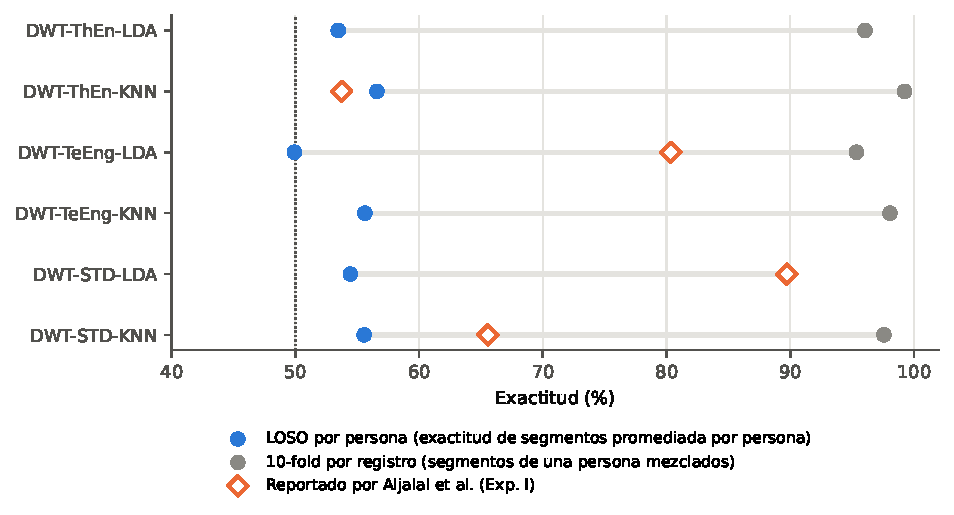
\includegraphics[width=0.92\linewidth]{../paper/figs/es_dev.pdf}
\caption{Mismas características y clasificadores. Azul: separando por persona. Gris: mezclando segmentos de la misma persona. Rombos naranjas: lo que reportó el artículo.}
\end{figure}

\begin{enumerate}[itemsep=3pt]
\item \textbf{Fuga entre segmentos.} Separando por persona, la exactitud es de 50 a 57\,\%: azar. Mezclando segmentos de la misma persona, de 90 a 99\,\%. El 89.7\,\% del artículo con todos los electrodos coincide casi exacto con nuestro 89.8\,\% mezclando segmentos. No podemos afirmar que ellos mezclaron, pero sus cifras son compatibles con eso.
\item \textbf{Sesgo de selección.} NSGA-II con diagnósticos al azar logra 72 a 79\,\% de exactitud ``interna'': lo mismo o más que con los diagnósticos reales. Con validación anidada, la combinación elegida con 23 personas da 67\,\% por dentro pero 40\,\% en la persona nueva.
\item \textbf{Ojos.} Fp1, Fp2, F7 y F8 están en la frente y captan los movimientos de los ojos (68\,\% de la señal de Fp1 y 39\,\% de la de F8). Dos de los electrodos favoritos del artículo son de esos. Si un grupo mueve más los ojos, el modelo detecta ``ojos'', no MCI.
\end{enumerate}

\section{Las mejoras que propusimos y por qué}

Cada mejora ataca uno de los problemas. Ninguna se eligió porque diera el número más alto.

\begin{center}\small
\begin{tabularx}{\linewidth}{@{}l>{\raggedright\arraybackslash}X>{\raggedright\arraybackslash}X@{}}
\toprule
Método & Qué es & Qué problema ataca \\
\midrule
R & Réplica fiel del artículo (DWT, entropía de umbral, 19 electrodos, NSGA-II, regla de quedarse con la mayor exactitud) & Es el punto de comparación \\
M0 & EEG limpio con ICA, sin los 4 electrodos frontales, potencia relativa en delta/theta/alfa/beta promediada por persona, LDA regularizado, 15 electrodos & Ojos, fuga entre segmentos (la unidad es la persona), sobreajuste (modelo simple y regularizado); usa medidas que la literatura asocia con MCI \\
M4 & Como M0, pero 1 electrodo por zona (frontal, central, temporal, posterior): 180 combinaciones posibles & Sesgo de selección: menos combinaciones, menos suerte \\
M1 & Como M0, con NSGA-II y la regla del artículo & Separa el efecto de la limpieza del efecto del algoritmo \\
M6 & Como M0, con enjambre de partículas (PSO) que castiga cada electrodo extra & Comprueba que la conclusión no dependa del algoritmo; premia la parsimonia \\
Físico & M0 y M4 sin referencia promedio ni ICA & Electrodos virtuales: ¿funcionaría con electrodos reales? \\
\bottomrule
\end{tabularx}
\end{center}

En desarrollo, estas versiones dieron cifras honestas (61 a 64\,\% con validación anidada), ninguna por encima del azar con 24 personas. Eso ya era una señal de alerta: la base es demasiado chica para demostrar nada.

\section{Cómo lo probamos: preregistro y prueba externa}

Usamos una segunda base pública del mismo hospital y el mismo equipo (\textbf{EEG\_2}, 34 personas: 18 con MCI y 16 sanas) que ningún método había visto.

\begin{enumerate}[itemsep=2pt]
\item \textbf{Congelamos} los cinco métodos y el análisis físico en el código.
\item \textbf{Extrajimos} las características de EEG\_2 sin entrenar nada, y les sacamos una huella digital (SHA-256). La extracción es exacta: repetirla da archivos idénticos bit a bit.
\item \textbf{Registramos en OSF} (\url{https://osf.io/4enh8}) las hipótesis, las reglas de decisión, el margen de 10 puntos y las huellas del código y de los datos.
\item \textbf{Corrimos la prueba una sola vez}, con un programa que aplica las reglas registradas automáticamente.
\end{enumerate}

Las hipótesis registradas fueron: \textbf{H1}, la réplica tendrá alta exactitud interna pero mucho menor en EEG\_2; \textbf{H2}, M0 no será peor que la réplica; \textbf{H3}, M4 y M6 no serán peores que M1 y usarán menos electrodos; \textbf{H4}, el montaje físico de M0 no será peor que con ICA.

\section{Qué salió}

\begin{figure}[h]
\centering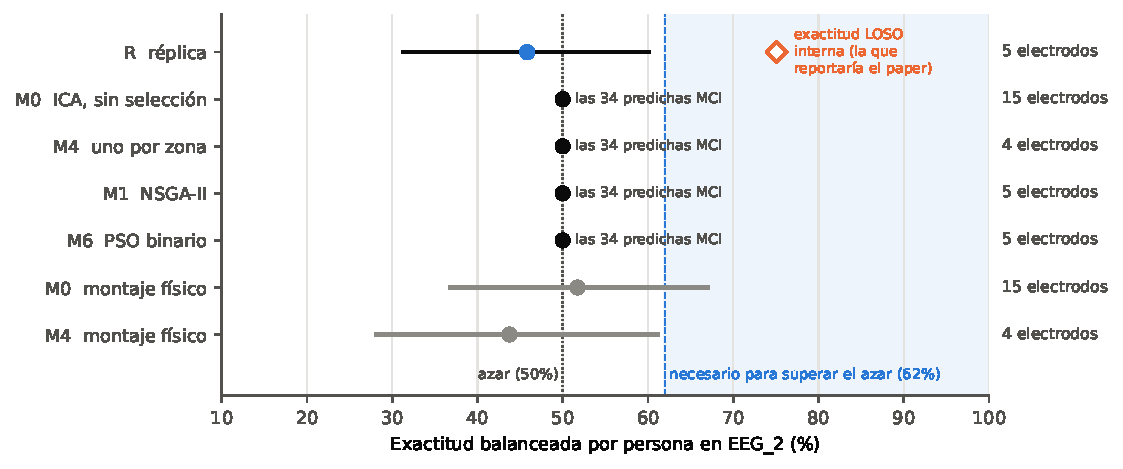
\includegraphics[width=0.95\linewidth]{../paper/figs/es_main.pdf}
\caption{Exactitud balanceada en las 34 personas nuevas. El rombo naranja es lo que la réplica ``creía'' tener por dentro.}
\end{figure}

\begin{itemize}[itemsep=3pt]
\item \textbf{H1 se confirmó.} La réplica eligió T3, Cz, T4, Pz y P4 (Cz y T4 coinciden con el artículo) y por dentro decía 75.1\,\%. En personas nuevas obtuvo 45.8\,\% (IC 31 a 60\,\%): por debajo del azar.
\item \textbf{Ningún método superó el azar.} Los cuatro métodos limpios dijeron ``MCI'' a las 34 personas. Por eso su exactitud balanceada es exactamente 50\,\%.
\item \textbf{H2 y H3 se cumplieron, pero de forma trivial.} Como los métodos dicen lo mismo para todos, ``no son peores'' que la réplica ni entre sí. Eso no demuestra que funcionen, y el artículo lo dice así.
\item \textbf{H4 fue no concluyente.} Los intervalos incluyen tanto la pérdida de 10 puntos como el cero.
\end{itemize}

\section{Por qué fallaron}

\begin{figure}[h]
\centering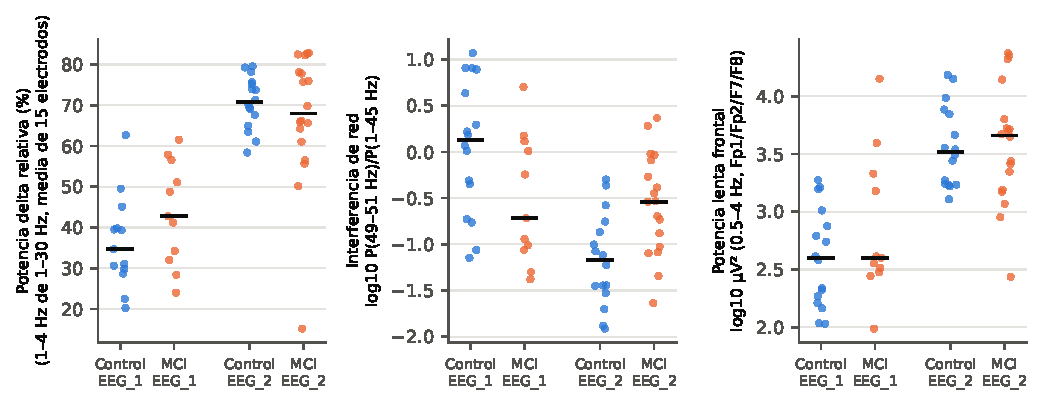
\includegraphics[width=0.98\linewidth]{../paper/figs/es_conf.pdf}
\caption{Cada punto es una persona. Las diferencias entre bases son más grandes que entre MCI y sanos.}
\end{figure}

\begin{enumerate}[itemsep=3pt]
\item \textbf{Las dos bases se distinguen casi perfecto.} Solo con el EEG se sabe de qué base viene una persona con 94.4\,\% de exactitud, aunque ambas son del mismo hospital y equipo.
\item \textbf{EEG\_2 está dominada por ondas lentas.} En EEG\_2 la banda delta es el 69\,\% de la potencia; en EEG\_1, el 40\,\%. En EEG\_1 los MCI tenían un poco más de delta que los sanos, así que los modelos aprendieron ``más delta = MCI''. En EEG\_2 todos tienen más delta que cualquiera de EEG\_1, y por eso todos salen MCI. Además, dentro de EEG\_2 la relación se invierte.
\item \textbf{El ruido de la red eléctrica engaña.} El ruido de 50\,Hz se relaciona con el diagnóstico en las dos bases, pero al revés: en EEG\_1 los sanos tienen más ruido; en EEG\_2, los MCI. Eso indica que las condiciones de grabación están mezcladas con los grupos.
\item \textbf{No hay señal escondida.} Ni el AUC (0.40 a 0.52), ni entrenar con las 27 personas, ni estandarizar cada base por separado revelaron una señal útil. El control positivo (menos alfa posterior en MCI) apunta en la dirección esperada pero es muy débil.
\end{enumerate}

\section{Entonces, ¿sirvieron las mejoras?}

Depende de qué se espere de ellas. \textbf{No} crearon una señal que no existe en estos datos; ningún método puede hacer eso. \textbf{Sí} cumplieron su función: dieron estimaciones internas honestas (nunca prometieron 95\,\%), no fueron peores que el método original y sus electrodos fueron estables entre semillas. La lección es que la estabilidad no es validez: un método puede elegir siempre los mismos electrodos y aun así estar ajustado a algo que no es la enfermedad.

\section{Qué aporta este trabajo}

\begin{enumerate}[itemsep=2pt]
\item Una réplica independiente del método, con código abierto (no encontramos otra publicada).
\item Una prueba externa preregistrada, con huellas digitales de código y datos, que el artículo original no tenía.
\item La medición de por qué las cifras salen altas (fuga, sesgo de selección, ojos) en lugar de solo afirmarlo.
\item El hallazgo de un cambio de dominio enorme entre dos bases del mismo hospital, y de un confusor de adquisición (ruido de red) que cambia de sentido.
\item La comparación entre electrodos virtuales y físicos, que casi nunca se reporta.
\item Un protocolo mínimo para futuros estudios de minimización de electrodos.
\end{enumerate}

\section{Limitaciones}

Las muestras son pequeñas: con 34 personas solo se detectan efectos grandes. No pudimos verificar que EEG\_2 use exactamente los mismos criterios de diagnóstico que EEG\_1, ni saber por qué tiene tanta actividad lenta (puede ser somnolencia, mala impedancia de electrodos o filtros distintos). Probamos la mejor configuración de selección de canales del artículo, no todas sus combinaciones. Solo usamos los primeros 10 minutos y no había datos de edad ni sexo. La estandarización por base se decidió después de ver los resultados y está marcada como \emph{post hoc}.

\section{Preguntas que podría hacer un revisor}

\begin{description}[style=nextline,leftmargin=0.4cm,itemsep=3pt]
\item[¿No será que su réplica está mal hecha?] La réplica reproduce el patrón del artículo: con segmentos mezclados obtiene cifras del mismo orden (89.8\,\% frente a 89.7\,\%), y su selección elige electrodos que coinciden con los del artículo (Cz y T4). Además, el código es público y da resultados idénticos en dos computadoras.
\item[¿Por qué no ajustaron el modelo a EEG\_2?] Porque entonces EEG\_2 dejaría de ser una prueba independiente. Aun así, como análisis \emph{post hoc}, estandarizamos cada base por separado y no apareció señal.
\item[¿H2 y H3 confirmadas no son un éxito?] No: se cumplen porque los métodos predicen lo mismo para todos. El artículo lo explica para no venderlo como éxito.
\item[¿Y si con más personas sí funciona?] Es posible que exista un efecto pequeño; el control positivo apunta en la dirección esperada. Pero no es el 95\,\% reportado, y para encontrarlo haría falta una base más grande y homogénea, con validación externa.
\item[¿Por qué preregistrar si los datos ya existían?] Porque lo que importa es que el análisis no se ajuste después de ver los resultados. Lo declaramos con honestidad: la base de desarrollo sí se había analizado, la de prueba no.
\end{description}

\section{Dónde está cada cosa}

\begin{itemize}[itemsep=1pt]
\item Preregistro: \url{https://osf.io/4enh8}.
\item Artículo en inglés y en español (PDF y LaTeX), póster en ambos idiomas, carta al editor, lista de verificación y repositorio de código: dentro del archivo zip.
\item Datos: \url{https://misp.mui.ac.ir/en/eeg-data} (Kashefpoor et al., 2016 y 2019).
\end{itemize}

\end{document}
